\section{Diskussion der Ergebnisse}

\subsection{Unterschiede in Kontrolle und Transparenz}
Die Auswertung der Fallstudie zeigt, dass Kontrolle und Transparenz über persönliche Daten und freiwillige Daten zwischen den Diensten stark variieren. Weiterhin wird das Nutzerverhalten und das Kaufverhalten ausgewertet.

- Kontrolle/Transparenz variiert stark von Dienst zu Dienst
    *Weiterverarbeitung
    *Entfernen von Daten
    *zum Teil kann man der Aufzeichnung des Nutzerverhalten/ Kaufverhalten von Personen für die Marketingzwecken widersprechen

- Validierung der pers. Daten für Kunsomenten: 
    *BitsAboutMe Abgleich Konto vs Kassenzettel
    *Datum Trust-Ranking-System gut, aber noch offen
- BitsAboutMe und Invisibly sehr ähnlich aber trotzem unterschiedlich
- BAM und Invisibly VS Datum
-Basisdaten werden bei Bonusprogrammen verarbeitet, wer freiwillige Angaben angibt, so werden diese auch verarbeitet (Kontrolle erfolgt über Bestätigungslinks oder durch Zusendung von Werbung auf dem postalischen Wege)
=> ergebnis man kann sie nicht kategoriesieren, alle sind "einzigartig"


- Motivation für Kunden:
    * BAM Analyseservices
    * Invisibly persönliches Feed, nicht manipulativ
    * Coupons, Rabatte, bares Geld (Anreiz)
- Lock-In Effekte
    * Bonusprogramme stark
    * Bei Brokern eher schwach
- Anreiz bewerten: Daten preiszugeben für Gegenwert

- Wert der Daten bzw. Wert für Kunden schlecht vergleichbar und schwer zu bestimmen
    * Dienste in unterschiedlichen Stadien (Fertig, Beta, Konzepte)
    * teilweise nicht praktisch testbar
    * unterschiedliche Preismodelle für Datensätze (BAM dynamisch, Invisibly flat)
    *bei Bonusprogrammen erzielt man mehr durch das Kaufverhalten Werte, als durch persönliche Angaben

- Generelle Probleme:
    * Plattformen können Missbrauch nicht verhindern, d.h. Konsumenten können Daten weiterverwenden oder verkaufen => Daten nicht rückrufbar
    * Andere Dienste können weiterhin Daten sammeln und verkaufen (Kontrolle auf Plattform vs. Kontrolle bei Datenquelle)
    * Scope: Händlergebunden vs. Breit Verfügbar
    * Daten werden lange aufgehoben

- Erkenntnis:
    * Personen beteiligen sich zwar, aber verkaufen nicht aktiv auf knopfdruck Daten
    * Eher Daten bereitgestellt und warten auf Angebote von Käufern
    * Dennoch aktive Teilnahme an der Datenökonomie, durch evtl. Zustimmung des Nutzers zu Marketingzwecken und damit sein Kaufverhalten
    * Personen werden dazu animiert die Daten zu verkaufen, um damit etwas Geld zu verdienen
    * zudem werden Personen dazu animiert durch Rabatte und Coupons etwas zu kaufen, was sie ohne diese nicht tun würden.


    \subsection{Bonusprogramme}

    Mit der Recherche nach Payback und Cashback Programmen hat sich gezeigt, dass diese bereits unter dem Begriff Bonusprogramme zusammengefasst werden.\newline
    
    \noindent Bei Payback werden Treuepunkte gesammelt, die anschließend ab einer gewissen Punkteanzahl in Gutscheine bzw. Voucher, Rabatte, Coupons und Prämien eingelöst werden können. Zum Beispiel bei Fluglinien können Personen Flugmeilen sammeln, welche für Freiflüge, Upgrades, Hotelübernachtungen oder Mietwagen eingelöst werden können. Bei Payback bleibt das Geld bzw. die Leistung im Kreislauf des beteiligten Unternehmens. \cite{paycashback_all} \newline
     
    \noindent Beim Cashback bekommt der Kunde bares Geld zurück, welches er woanders wieder investieren kann. Cashback Anbieter erhalten eine Provision durch sogenannte Affiliate Links, in dem über das Portal der Verkauf bestätigt wird. \cite{cashback-vergleich} \newline
    
    \noindent Für den Erhalt des Geldes muss der Kunde/ Teilnehmer seine Kontodaten bekanntgeben. \cite{paycashback_all} \newline
        
    
    \begin{figure}[!ht]
        \centering
        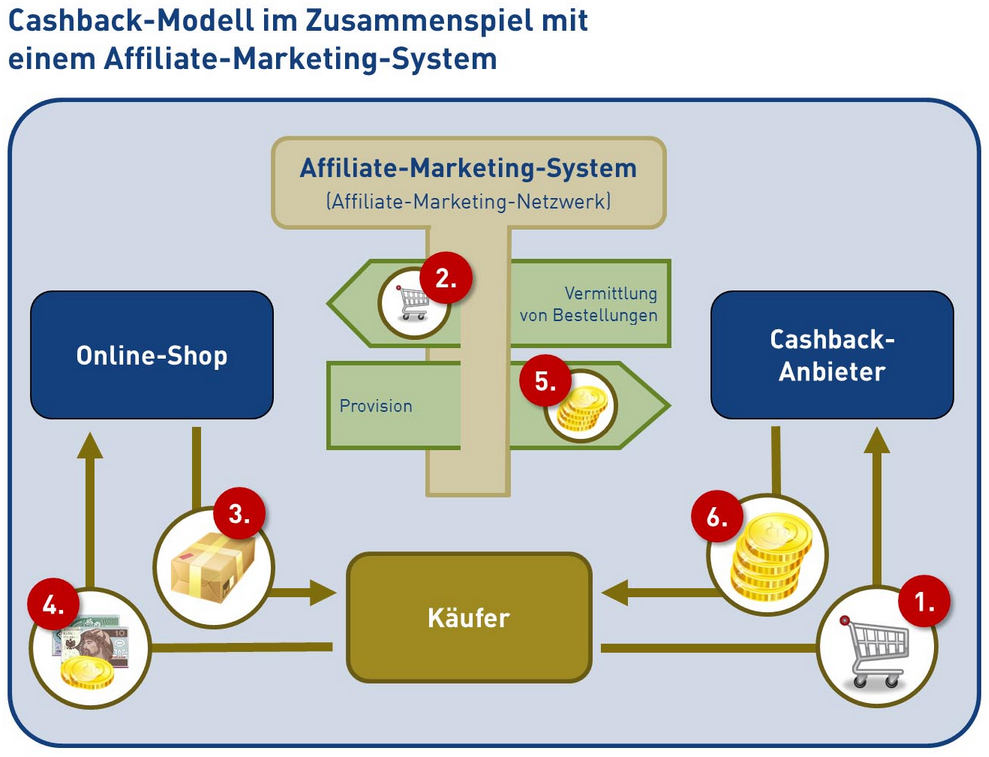
\includegraphics[width=0.8\textwidth]{Cashback-Modell im Zusammenhang mit einem Affiliate-Marketing-System}
        \caption{Cashback-Modell im Zusammenhang mit einem Affiliate-Marketing-System \cite{Bonus_affiliate} }
        \label{fig:Bonus_affiliate}
    \end{figure}
    \FloatBarrier
    
    Die Abbildung 4.1 zeigt den Ablauf des Affiliate Marketing Systems. Das bedeutet der Kunde sieht zum Beispiel auf einem Blog einen Artikel, welchen er gerne erwerben möchte, dazu klickt er einfach auf den sogenannten Affiliate Link (1). Dieser führt zum Onlinehändler, wo der Kunde diesen Artikel erwerben kann (2). Anschließend versendet der Shop die Ware an den Käufer (3). Danach bezahlt der Käufer seine Ware beim Onlineshophändler (4). Nachdem der Käufer seine Ware bezahlt hat, zahlt der Onlinehändler eine Provision an den Cashback-Anbieter (5). In diesem Beispiel wäre das der Besitzer des Blogs. Nachdem der Cashback Anbieter die Provision erhalten hat, zahlt er an den Käufer einen gewissen Prozentsatz an den Käufer aus (6). \cite{Bonus_affiliate} \newline

    \noindent Der wesentliche Unterschied zwischen Cashback und Payback liegt darin, das mit Cashback direkt nach jedem Einlauf Geld erstattet wird, welcher auf das Bankkonto des Kunden gutgeschrieben wird. Dies kann über Affiliate Links oder auch über Kassenzettel einsenden geschehen. Zum Beispiel gibt es Aktionen 3 für 2 (1x wird direkt ausgezahlt) im Einzelhandel von Weichspüler oder Schokolade. Dazu muss man in dem Aktionszeitraum die Produkte einkaufen und anschließend den Kassenzettel hochladen. Danach bekommt der Käufer das Geld erstattet, welches zuerst vom Kunden ausgegeben wurde. Payback kann erst im Anschluss ab einer gewissen Punktemenge in Prämien, Gutscheine, Rabatte oder Coupons eingelöst werden. \cite{TreueCash} \newline
    
    \noindent Es existieren noch viele weitere verschiedene Anbieter für Bonusprogramme, als die in der Fallstudie aufgezeigten Beispiele. Zum Beispiel für Treuepunkte sei genannt DeutschlandCard, Payback, Webmiles, KauflandCard, DM. Für Cashback-Programme z. B. card4you, Shoop. \newline

    \noindent Grundsätzlich sei genannt, dass die Bonusprogamme die nachfolgenden Ziele verfolgen:\newline
    - Kundenbindung \newline
    - Kundendaten erheben und auswerten \newline
    - Kundenbindungsprogramme steigern den Umsatz durch neue Kunden \cite{paycashback_all} 
